\documentclass{article}
\usepackage{amsmath, amssymb, amsfonts}
\usepackage{fullpage}
\usepackage{enumerate}
\usepackage[linesnumbered,ruled,vlined]{algorithm2e}
\usepackage[usenames,dvipsnames]{xcolor}
\usepackage[colorlinks,allcolors=RoyalBlue]{hyperref}
\usepackage{enumitem}
\usepackage{graphicx} % Required for inserting images
\usepackage[margin=1in]{geometry}
\usepackage{xcolor}
\usepackage{amsmath}
\usepackage{tikz}
\usepackage{tkz-base}
\usepackage{tkz-euclide}
\usepackage{comment}
\usepackage{booktabs}
\usepackage{graphicx}
\usepackage{adjustbox}
\graphicspath{ {./images/} }

% Grading
% There is not a specific grading rubric for the project report. However, we will look for the following factors:
% How much thought and consideration did you put into the problem setting? Is the problem setting sufficiently challenging or interesting to explore?
% How much thought and consideration did you put into your approach? Did you correctly identify the previous approaches and their limitations? Did you attempt to address theses limitations through your work? Did you note key obstacles in implementing your approach? Even if your results were not successful, did you try enough things and reflect on why they did not work? What would you have done differently given more time and resources?
% How much thought and consideration did you put into your investigation? Did you use reasonable performance metrics? Did you provide insight and visualize key aspects of your approach (using tables, figures, toy examples)? For any theoretical components of the project, have you identified the crucial assumptions and limitations?

\font\myfont=cmr12 at 15pt
\title{\vspace{0cm}\myfont CS 4782 Final Report}
\author{Sunny Sun, Michael Wei, Tony Chen, Linda Hu, Jiye Baek}

\begin{document}

\maketitle

\section{Introduction}

% State the problem and motivation.
% Include the title and authors of the paper (if reproducing one).
% Summarize the primary method and contributions of the paper.

In this project, we aimed to reproduce the image captioning results of the paper \textit{Show, Attend, and Tell} published in 2016 by Kelvin Xu \textit{et al}. This paper utilizes the then novel technology of attention to create more accurate and efficient methods of automatic caption generation of a given input image. This paper was motivated by the computer vision problem of determining not only what objects exist within an image, but also accurately describing the relationships between them in a natural language.

Although prior image-captioning networks existed at the time this paper was written, most used static global image features which often miss fine-grained spatial details crucial for accurate captioning. This paper's main contributions include introducing two attention-based image caption generators under a common framework, visualizing the results of this framework by outputting alpha masks that depict the area of an image that the attention focused on, and quantitatively validating the usefulness of attention in caption generation using standard metrics of BLEU and METEOR scores.

\section{Chosen Result}

% Identify the specific result you aimed to reproduce and its significance in the context of the paper’s main contribution(s).
% Include the relevant figure, table, or equation reference from the original paper.
% State why it was chosen and its importance in the context of the paper or your goals.

Besides implementing the underlying infrastructure of the model outlined in the paper, we aimed to reproduce two main results:

\textbf{Visualization of soft attention} at each timestep of a generated caption. The original paper has several examples of the change in attention over time to reflect the relevant parts of the image. We chose this visualization to understand the attention mechanism used by the model and gain intuition into what the model saw.

\begin{figure}[h]
    \centering
    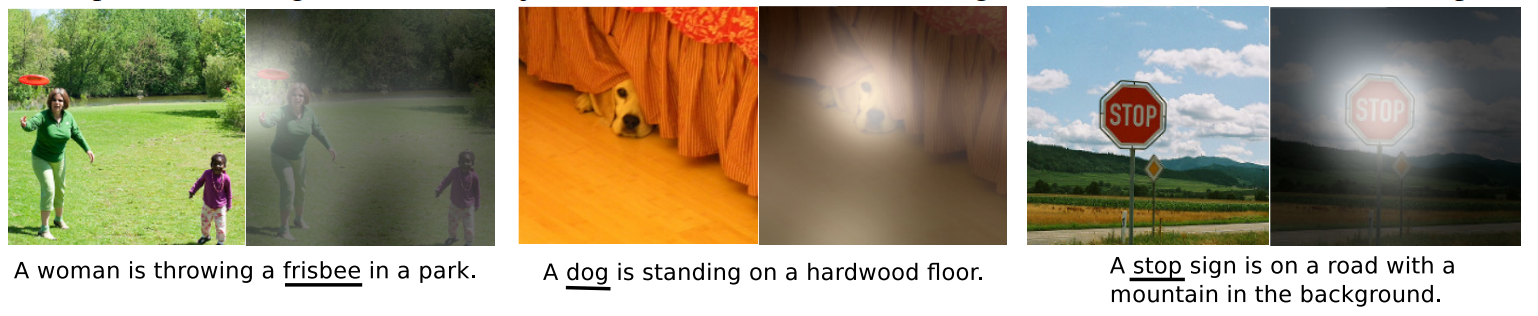
\includegraphics[width=0.9\linewidth]{chosen-results.png}
    \caption{Visual examples of soft attention from the original paper}
    \label{fig:results}
\end{figure}

\textbf{BLEU and METEOR scores} reported for the soft attention model on the Flickr8k dataset. These are common metrics used in natural language processing that quantitatively evaluate the quality of generated captions against human understanding. We chose these results to provide a concrete standard from which we can measure the accuracy of our model.


\section{Methodology}
\begin{figure}[h]
    \centering
    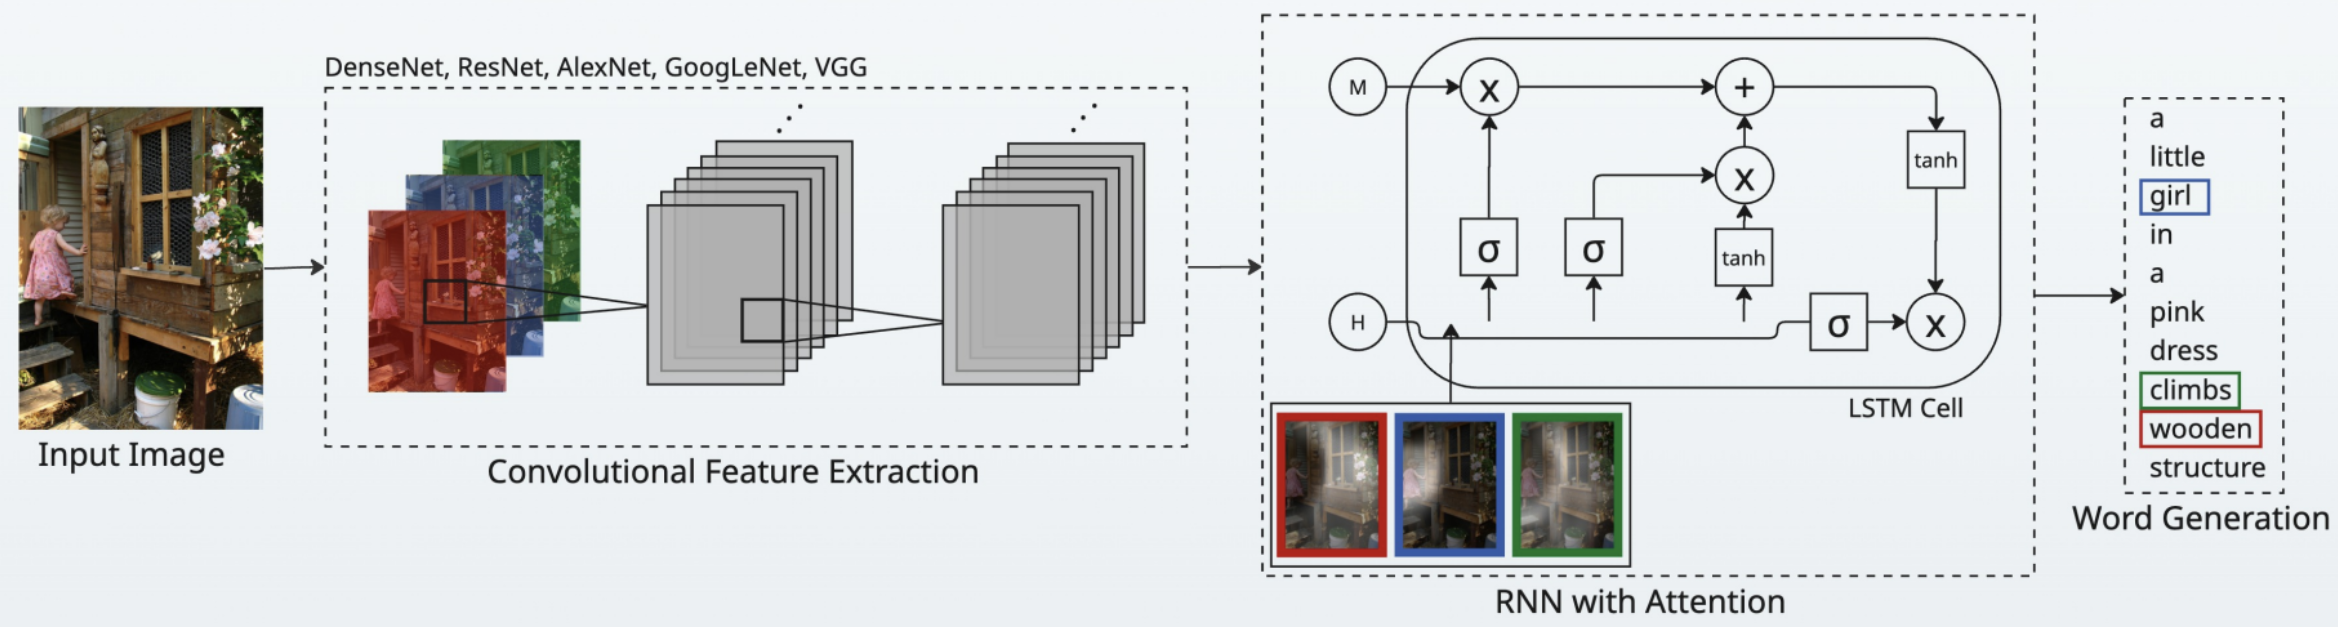
\includegraphics[scale=0.2]{methodology.png}
    \caption{Overall Model Architecture}
    \
\end{figure}
The model takes in a single raw image and passes it through a convolution neural network (CNN) encoder such as VGG, ResNet, or DenseNet to extract spatial image features in annotation vectors. Instead of training from scratch, we used frozen, pre-trained CNNs encoders to experiment with newer architectures and save compute. We used the encoders from the original paper --- VGG, GoogLeNet, and AlexNet --- for consistency and baseline comparison. To evaluate the impact of more recent architectures, we also included ResNet and DenseNet, which were introduced after the paper was published. ResNet, with its skip connections, addresses the vanishing gradient problem and enables stable training of deeper networks. DenseNet uses dense connections to promote feature reuse and improve generalization. These design improvements allow both models to capture complex patterns, which likely contributed to their stronger performance, even on our smaller dataset.

The attention model calculates the weights for each annotation vector. These are used in attention mechanism to generate a context vector, indicating where in the image the model attends to at that timestamp. The paper uses two types of attention: hard and soft attention. Soft attention calculates the expected value of all annotation vectors using the softmax of the weights, whereas hard attention uses the weights for each annotation vector to create a multinoulli distribution which is then sampled. Then, hard attention samples from each location of the image as one-hot variable--1 if the i-th location of the image is used to extract visual features, else 0. Thus, the context vector in the hard attention implementation is a multinoulli distribution. We ultimately chose to omit the implementation of hard attention due to its reliance on reinforcement learning, which introduces additional complexity and instability during training. 

In the LSTM decoder, we initialized the memory state and hidden states by taking the average of the annotation vectors fed through 2 MLPs. The context vector, previous word, and previous hidden state are fed into LSTM decoder at every word predicted in the caption.

The original paper trained the soft attention model on MS COCO for 3 days on an NVIDIA Titan Black GPU. We trained our re-implemented model over 20 epochs using Adam optimizer with a learning rate of 0.0001 and a batch size of 32. Due to time and memory constraints, we only trained our model on the Flickr8k dataset alone, avoiding Flickr30k and MS COCO in the paper. The smaller dataset also allowed us to maintain fast experimentation cycles and train our model in around 2 hours. We used the train, val, test labels in the dataset to split our data. This gave us 6000 images for the training set and 1000 images each for the validation and test set. In the dataset, there are 5 human annotated captions per image. To evaluate our caption quality, we used BLEU and METEOR scores to calculate the training and validation accuracy. We calculated these scores for soft attention alone, but across all 5 pretrained CNN encoders.

% Describe your re-implementation approach, including the model architecture, datasets, evaluation metrics, and any modifications made to the original methodology.

\section{Results and Analysis}

% Present your re-implementation results and compare them to the original paper’s findings. 
% Discuss any discrepancies or challenges encountered during the re-implementation process.
% Provide an analysis of your results in the context of the paper’s main contribution(s) and the broader research area.
% Note: We are looking for a reasonable re-implementation of the method and a clear discussion of your results. A failure to match the reported results could happen for any number of reasons that would not negatively impact your grade. It is acceptable, for instance, to run smaller-scale experiments if you initially under-estimated the required resources for your selected result. It’s also possible that the authors left out some detail that is necessary to match their performance.

In terms of BLEU and METEOR scores, our re-implementation achieved slightly lower compared to the original paper's soft attention scores for the Flickr8k dataset. We also trained the model with various frozen, pre-trained encoders and found that ResNet performed the best. However, in the original paper, the model fine-tuned its encoders during training, which may account for the discrepancy between our model's and the original paper's BLEU and METEOR scores. The scores of our models and the original paper are shown in the table below.

\begin{table}[h]
\centering
\begin{adjustbox}{width=.75\textwidth}
\small
\begin{tabular}{lccccc}
\toprule
Model & BLEU-1 & BLEU-2 & BLEU-3 & BLEU-4 & METEOR \\
\midrule
Soft-Attention (Original Paper) & 67.0 & 44.8 & 29.9 & 19.5 & 18.93 \\
AlexNet                & 60.44 & 34.90 & 19.71 & 10.81 & 12.89 \\
DenseNet               & 64.81 & 40.82 & 26.26 & 15.84 & 16.95 \\
GoogLeNet              & 64.53 & 40.13 & 25.12 & 14.77 & 16.45 \\
VGG                    & 64.79 & 40.37 & 25.88 & 15.48 & 17.08 \\
ResNet                 & \textbf{65.67} & \textbf{41.40} & \textbf{27.13} & \textbf{16.48} & \textbf{17.94} \\
\bottomrule
\end{tabular}
\end{adjustbox}
\end{table}

In terms of visualization and qualitative performance, we fed several random images to our model and obtained captions and attention maps after training. We can see in words such as "drive" and "is" that the model is able to attend to salient regions for even words that are non-object. The model learns alignments that correspond pretty strongly to human intuition, similar to the original paper's findings. Based on the generated attention masks, we would claim that our re-implemented model is capable of building a coherent visual-linguistic representation, grounding each word in relevant spatial context. 

\begin{figure}[h]
    \centering
    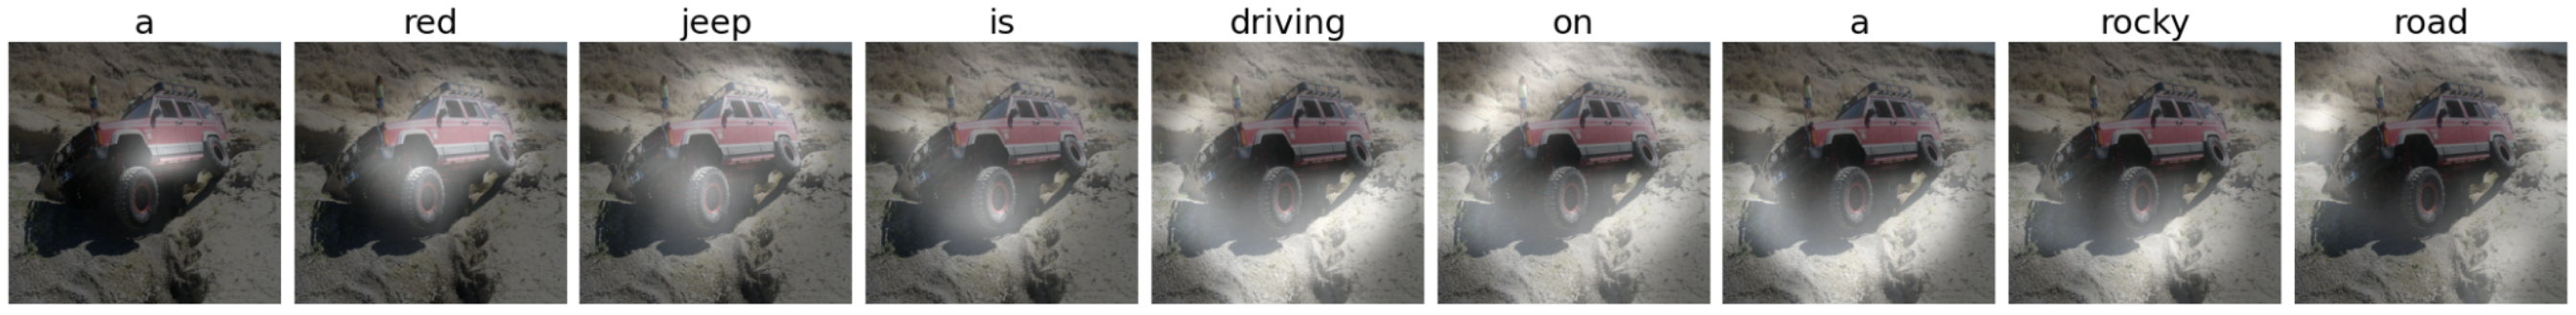
\includegraphics[width=0.75\linewidth]{example-jeep.png}
    \caption{Example of our model's attention mechanism visualization per word in generated caption.}
    \label{fig:enter-label}
\end{figure}

One challenge that we faced in the re-implementation process was long training times and timing out on compute while using a T4 GPU on Google Colab. On average, training 10 epochs would take almost two hours. We partially resolved these problems by optimizing the decoder of the model. We also implemented saving model checkpoints at every epoch so we could break up training time over multiple sessions.

\section{Reflections}

% Share lessons learned during the project.
% Summarize the key takeaways from your re-implementation effort and the lessons learned.
% Discuss potential future directions or extensions based on your findings and the paper’s implications.

Our re-implementation demonstrated meaningful results given limited resources. Despite only training on the smaller Flickr8k dataset and using frozen pre-trained CNN encoders, our model generated reasonable captions and produced interpretable attention maps. This highlights the effectiveness of the soft attention mechanism, even under constraints.

One of the key lessons we learned was the importance of feasibility given time constraints and tight resources. Although the original paper explored both hard and soft attention mechanisms, we found that soft attention was significantly more practical to implement and train due to its differentiable and deterministic nature. Implementing the hard attention, especially the required reinforcement learning techniques like REINFORCE, from scratch was more time consuming than anticipated.

Overall, this project deepened our understanding of attention mechanisms in image captioning and provided practical experience in re-implementing a significant paper in computer vision and natural language processing. For potential future work and with more time and computational capacity, we would look into using larger datasets that the original paper used such as Flickr30k and MS COCO to improve generalization and caption quality. We can also try to implement hard attention mechanism using REINFORCE to explore sharper spatial focus. Finally, we can fine-tune CNN encoder during training to allow the model to learn image features more tailored to caption generation.


\section{References}

% Include full citations for the original paper and any tools, datasets, or frameworks used.
[TODO DO WE NEED TO CREDIT MORE TOOLS ??]
\begin{itemize}
    \item Xu, K., Ba, J., Kiros, R., Cho, K., Courville, A., Salakhutdinov, R., Zemel, R., \& Bengio, Y. (2015). Show, Attend and Tell: Neural Image Caption Generation with Visual Attention. Paper Website. \\ https://kelvinxu.github.io/projects/capgen.html
    \item Xu, K. Arctic Captions: Theano Implementation of Show, Attend and Tell. GitHub repository. https://github.com/kelvinxu/arctic-captions 
    \item Wong, A.. Show, Attend and Tell: PyTorch Implementation. GitHub repository. \\ https://github.com/AaronCCWong/Show-Attend-and-Tell
    \item Hodosh, M., Young, P., \& Hockenmaier, J. (2013). Framing Image Description as a Ranking Task: Data, Models and Evaluation Metrics. Journal of Artificial Intelligence Research, 47, 853–899.\\ https://doi.org/10.1613/jair.3994
    \item Paszke, A., Gross, S., Massa, F., Lerer, A., Bradbury, J., Chanan, G., ... \& Chintala, S. (2019). PyTorch: An Imperative Style, High-Performance Deep Learning Library. Advances in Neural Information Processing Systems, 32. \\ https://arxiv.org/pdf/1912.01703
\end{itemize}

\end{document}
